\documentclass[11pt]{article}
\usepackage[margin=1in]{geometry}
\usepackage{amsmath,amssymb,amsthm,booktabs,pgfplots}
\usepackage{flafter,placeins}
\usepackage[hidelinks]{hyperref}
\pgfplotsset{compat=1.18}
\newtheorem{proposition}{Proposition}
% Load generated row definitions before entering the table alignments.
\newcommand{\SizeRows}{%
8 & 4/560 & 2.83 & 3.30 & 0.323 \\%
16 & 50/1,200 & 4.01 & 4.79 & 0.326 \\%
32 & 241/2,480 & 5.02 & 6.09 & 0.342 \\%
64 & 1,134/5,040 & 7.35 & 8.58 & 0.407 \\%
}

\newcommand{\FamilyRows}{%
Erd\H{o}s--R\'enyi & 6.64 & 8.04 & 10.09 & $+1.40\pm1.69$ \\%
Grid & 41.62 & 43.91 & 46.52 & $+2.28\pm2.52$ \\%
Cycle & 76.78 & 78.88 & 82.87 & $+2.10\pm2.75$ \\%
Path & 106.78 & 108.83 & 112.86 & $+2.05\pm2.75$ \\%
}

\newcommand{\PathRows}{%
Center & 7.97 & 6.71 & 13.94 & 10.52 \\%
Endpoint & 29.75 & 26.92 & 26.18 & 19.68 \\%
}

\title{Neural Algorithmic Reasoning:\\ Generalization and Theoretical Limitations of Graph Neural Networks}
\author{Zidane Boussofi}
\hypersetup{pdfauthor={Zidane Boussofi}}
\date{}
\begin{document}
\maketitle
\begin{abstract}
We study weighted single-source shortest-path regression with synchronous graph neural networks trained on final distances. Across five paired replicates, raw mean absolute error increased with graph size for all six configurations on connected Erd\H{o}s--R\'enyi graphs. For the standard four-round model, normalized error rose from 0.323 at 8 vertices to 0.407 at 64. We specialize standard message-passing locality to weighted shortest-path prediction and construct path queries that force identical predictions for different exact distances. In a controlled 24-vertex path study, eight rounds reduced mean error on both source probes with near-matched parameter and dense-operation counts. Endpoint training improved endpoint predictions and degraded center predictions. Improvements beyond source reach show that empirical error can decrease even where the source indicator cannot influence a prediction.
\end{abstract}

\section{Introduction and motivation}
A fixed-depth graph neural network can accept graphs of arbitrary size, but each prediction depends on a bounded number of propagation rounds. On synthetic graphs, we ask how error changes with size within a family and across families at matched size, whether extra rounds help newly reachable nodes, and whether residual updates improve transfer under a fixed training budget. Final-distance supervision leaves open whether the models execute intermediate steps of Dijkstra or Bellman--Ford. A source-swap analysis characterizes which queries the architecture can distinguish for any parameters.

\section{Related work}
Gilmer et al.\ formalized a common message-passing framework \cite{gilmer}. Xu et al.\ related neighborhood aggregation expressivity to the Weisfeiler--Lehman test and identified limitations of common aggregators \cite{xu}. Our locality proposition uses isomorphic attributed balls as a sufficient condition for equality. It makes no injectivity assumption about aggregation. Yehudai et al.\ studied size generalization when local structure changes with graph size \cite{yehudai}. Our connected random-graph series also changes distances and coverage as size grows.

Veli\v{c}kovi\'c et al.\ trained neural models to imitate intermediate steps of graph algorithms \cite{execution}. The CLRS benchmark provides a common framework for learning across classical algorithms \cite{clrs}. Here Dijkstra provides exact targets \cite{dijkstra}, and the model receives final-output supervision. Oversmoothing concerns loss of representational distinctions under repeated propagation, as studied under specific spectral conditions by Oono and Suzuki \cite{oono}. Oversquashing concerns compressing long-range information into limited representations \cite{alon}. Neither mechanism was measured here. The proof below concerns absence of an input dependency before any signal can arrive.

\section{Mathematical background}
Let \(G=(V,E)\) be finite, simple, connected and undirected, with weights \(w:E\to\{1,\ldots,10\}\) in the experiments. For source \(s\), the target \(d_w(s,v)\) is the minimum total weight over paths from \(s\) to \(v\). Hop distance \(d_H(s,v)\) minimizes the number of edges. These minimizers can differ. Write \(B_k(v)\) for the rooted induced subgraph on vertices at hop distance at most \(k\) from \(v\).

\section{Models and experimental methodology}
The encoder maps the binary source flag to a state \(h_v^0\). Each undirected edge is represented in both directions, each with input \(w_{uv}/10\). For round \(t\), the message and update maps \(M_t,U_t\) are separate two-layer perceptrons with an intermediate ReLU. With shared parameters across vertices,
\[
a_v^t=\sum_{u\sim v}M_t(h_u^t,w_{uv}/10),\qquad
h_v^{t+1}=U_t(h_v^t,a_v^t)+\rho h_v^t ,
\]
where \(\rho=0\) for standard models and \(\rho=1\) for residual models. An affine readout forces the source prediction to zero using its local flag. The model has no positional identifiers, graph normalization or global broadcast. Hop counts are evaluation metadata.

One Adam step per graph minimizes non-source MAE on targets scaled by ten, using learning rate \(10^{-3}\). The earliest epoch attaining minimum validation MAE supplies the selected weights.

For an evaluation graph \(G=(V,E)\) queried at source \(s\), let
\(V_s=V\setminus\{s\}\) and \(n_s=|V_s|\). Write \(\hat d_v\) for the
predicted distance to vertex \(v\) in weight units, and let
\(e_v=|\hat d_v-d_w(s,v)|\) for \(v\in V_s\). The metrics for this graph and source are
\begin{align*}
\mathrm{MAE}(G,s) &= \frac{1}{n_s}\sum_{v\in V_s} e_v, \\
\mathrm{RMSE}(G,s) &= \sqrt{\frac{1}{n_s}\sum_{v\in V_s} e_v^2}, \\
\text{normalized MAE}(G,s) &= \frac{\sum_{v\in V_s} e_v}{\sum_{v\in V_s} d_w(s,v)}.
\end{align*}
Within each evaluation cell, take the arithmetic mean of each metric over
graphs in a replicate, then average those replicate means equally. Hop-band MAE pools nodes within a replicate. Paired contrasts subtract within replicate and report the mean and sample standard deviation (SD) of those differences. These SDs include variation in training and graph draws.

\paragraph{Generalization study.}
Phase 3 used five replicates with training seeds 0--4 and data seeds 1000--1004. Train and validation sets comprised 64 and 16 separate connected Erd\H{o}s--R\'enyi graphs, respectively, split evenly between 6 and 8 vertices. Before rejection for connectivity, \(p=3/(n-1)\). Evaluation crossed four sizes (8, 16, 32, 64) with connected Erd\H{o}s--R\'enyi, path, cycle, and two-row grid families, with 16 graphs per cell per replicate. Weights are uniform independent integers and one source is sampled uniformly per graph. Weighted-isomorphic duplicates were screened before encoding. The width was 32 for all configurations, with 2, 4 or 8 rounds and 768 updates per fit. Architecture pairs at the same depth share initial parameters and graph order. Across depths, the number of parameters grows from 10,657 to 42,337. Constant baselines predict zero or the pooled non-source training-target mean.

\paragraph{Controlled path study.}
Phase 4 used standard models on 24-vertex paths with independent weights from the same law. Five replicates used training seeds 0--4 and data seeds 4000--4004. Each used 32 training, 16 validation and 16 test paths. Weight sequences canonicalized under reversal exclude duplicates across main-study splits and replicates. Each training path is queried either at vertex 11 (center) or vertex 0 (endpoint), with the same graph draws in both regimes. Both source positions are queried for validation and test. Selection uses the combined validation queries. Depth four uses width 32 and depth eight uses width 23. Each fit uses 640 updates. Within depth the two regimes share initialization and graph order.

\section{Generalization experiments}
Figure~\ref{fig:size} shows rising raw MAE for each configuration. For the standard four-round model, normalized MAE also increased (Table~\ref{tab:size}). Between 8 and 64 vertices, mean target distance rose from 8.66 to 17.10 and mean unweighted diameter from 3.25 to 8.26, alongside a realized mean degree change from 3.04 to 3.26. The size series measures these shifts jointly.

\begin{figure}[htbp]
\centering
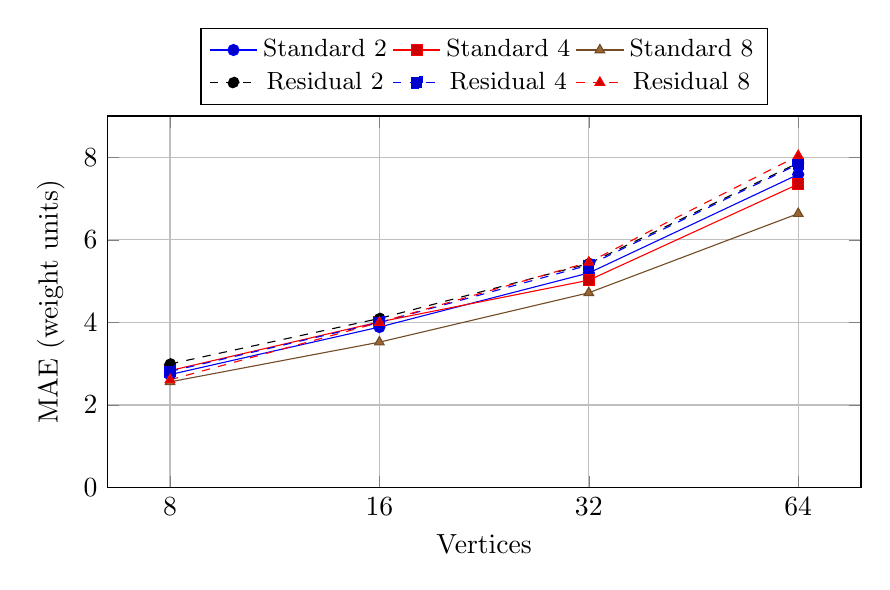
\begin{tikzpicture}
\begin{axis}[width=.92\linewidth,height=6.3cm,xmode=log,log basis x=2,
xtick={8,16,32,64},xticklabels={8,16,32,64},xlabel={Vertices},ylabel={MAE (weight units)},
ymin=0,ymax=9,grid=major,legend columns=3,legend style={font=\small,at={(.5,1.03)},anchor=south}]
\addplot+[solid,mark=*] coordinates {(8,2.735878) (16,3.887439) (32,5.197856) (64,7.584398)};
\addlegendentry{Standard 2}
\addplot+[solid,mark=square*] coordinates {(8,2.832394) (16,4.012128) (32,5.022922) (64,7.349770)};
\addlegendentry{Standard 4}
\addplot+[solid,mark=triangle*] coordinates {(8,2.559317) (16,3.521428) (32,4.717973) (64,6.636388)};
\addlegendentry{Standard 8}
\addplot+[dashed,mark=*] coordinates {(8,2.992782) (16,4.095315) (32,5.425351) (64,7.864447)};
\addlegendentry{Residual 2}
\addplot+[dashed,mark=square*] coordinates {(8,2.811810) (16,3.996305) (32,5.389106) (64,7.833700)};
\addlegendentry{Residual 4}
\addplot+[dashed,mark=triangle*] coordinates {(8,2.609835) (16,3.999161) (32,5.457113) (64,8.039847)};
\addlegendentry{Residual 8}

\end{axis}
\end{tikzpicture}
\caption{Mean graph-macro MAE over five replicates on connected Erd\H{o}s--R\'enyi graphs. Legend numbers give rounds. The 8-vertex cell anchors the in-distribution size comparison.}
\label{fig:size}
\end{figure}

At 8 vertices, standard depth-four MAE was 2.76 on grids, 2.83 on connected random graphs, 3.62 on cycles and 6.64 on paths. Every cycle query node was within four hops, and 120 of 560 path nodes exceeded four hops. At 64 vertices, differences in distance scale were substantial. Mean targets ranged from 17.10 on connected random graphs to 120.13 on paths. The family ordering reflects differences in degree, hop distribution and route redundancy as well as target scale.

Standard depth eight improved mean MAE relative to depth four in every 64-vertex cell. The residual model moved in the opposite direction. At depth eight the residual-minus-standard validation contrast was \(-0.05\pm0.23\), while the corresponding 64-vertex random-graph contrast was \(+1.40\pm1.69\) (Table~\ref{tab:family}). Thirteen of 30 fits selected the final epoch. For structured families, the standard-model mean improvement in the 9+ hop band was comparable to the improvement at 5--8 hops, with substantial paired variability. These depth comparisons also change capacity and computation per update.

\begin{table}[htbp]
\centering
\caption{Standard depth-four random-graph results. MAE and RMSE are in weight units. Counts pool five replicates.}
\label{tab:size}
\begin{tabular}{rrrrr}
\toprule
Vertices & Nodes beyond four hops & MAE & RMSE & Normalized MAE\\
\midrule
\SizeRows
\bottomrule
\end{tabular}
\par\medskip
\caption{Graph-macro MAE at 64 vertices in weight units. The last column is the paired residual-minus-standard mean and sample SD over five replicates.}
\label{tab:family}
\begin{tabular}{lrrrr}
\toprule
Family & Standard 8 & Residual 8 & Training mean & Residual contrast\\
\midrule
\FamilyRows
\bottomrule
\end{tabular}
\end{table}

% Keep generalization floats out of the propositions and proofs.
\FloatBarrier
\section{Theoretical locality results and proofs}
\begin{proposition}[Attributed neighborhood locality]
Suppose a deterministic model starts with a shared nodewise encoder, then performs \(k\) synchronous rounds of message passing on the original edges. Messages use previous endpoint states and fixed supplied oriented-edge attributes. Aggregation is permutation invariant over incoming messages. Updates are shared and may use the previous state, local node attributes and a residual addition. Readout is shared and nodewise. If two rooted \(k\)-hop balls are isomorphic with all supplied node and oriented-edge attributes preserved, their root outputs are equal under the same parameters.
\end{proposition}
\begin{proof}
Let \(f\) be an attribute-preserving rooted isomorphism between the balls. Distances to the root within each ball equal full-graph hop distances, since a shortest route to the root stays inside the ball. At time zero, corresponding states agree at every vertex of the balls by the encoder assumption. Assume at time \(t\) they agree for all corresponding vertices at distance at most \(k-t\). A vertex at distance at most \(k-t-1\) has every neighbor within distance \(k-t\). The rooted isomorphism therefore matches its complete incoming neighborhood, including attributes, previous endpoint states and the previous state of the receiver. The message multisets agree, so the aggregate and the updated states agree, including any residual addition. Induction gives equality at the roots after \(k\) rounds. The nodewise readout preserves equality.
\end{proof}

The assumptions exclude graph-wide inference statistics, virtual edges and broadcast pooling. If a model uses a sender's full degree, that value must be included as an attribute in the comparison, since a boundary sender may have neighbors outside the ball. The proposition is exact in real arithmetic. Reordering floating-point sums can introduce roundoff. The fixed-graph intervention preserves edge order.

\begin{proposition}[Shortest-path prediction error]
If the binary indicator is the only source-dependent input, then any two sources outside \(B_k(v)\) on the same graph yield the same prediction \(p\) at \(v\). For their targets \(a,b\), both the maximum and the equally weighted mean absolute errors are at least \(|a-b|/2\). At any fixed depth there are bounded-positive-weight graphs with arbitrarily large worst-case error as graph size grows.
\end{proposition}
\begin{proof}
The attributed balls agree because all their source flags vanish and all remaining attributes are fixed. The previous proposition implies the common prediction. The triangle inequality gives
\[
|a-b|\le |a-p|+|b-p|\le 2\max\{|a-p|,|b-p|\}.
\]
The midpoint attains both lower bounds. Take a unit-weight path on vertices \(0,\ldots,k+2\) and query sources \(k+1,k+2\) at vertex \(0\). Their targets are \(k+1,k+2\), yielding a bound of \(1/2\) weight unit. Extend the path to \(k+1+m\) and move the second source there. The attributes inside the ball still agree and the target gap is now \(m\). The lower bound grows without limit with \(m\).
\end{proof}

The bound concerns the constructed pair. If those observations are two of \(N\) equally weighted observations, their contribution to pooled MAE is at least \(|a-b|/N\). For normalized error on just the pair, the lower bound is \(|a-b|/(a+b)\). The earliest possible influence of the source flag is its hop distance, but even source visibility can be insufficient. On a triangle with prediction vertex \(v\), source \(s\) and third vertex \(u\), set \(w_{vs}=10\) and \(w_{vu}=1\). Increasing \(w_{us}\) from 1 to 9 changes the target from 2 to 10 while leaving the messages into \(v\) in round one unchanged.

\section{Targeted experimental validation}
All 30 Phase 3 main fits and all 20 Phase 4 main fits gave exactly equal CPU predictions on their constructed unit-path pairs, verifying the implementation on those inputs. The held-out path test measures regression error on randomly weighted paths.

Depth eight reduced overall mean MAE under each training regime on both probes (Table~\ref{tab:path}). The four- and eight-round models had 21,217 and 22,150 parameters and required 679,168 and 703,616 forward dense multiply-accumulates per query, respectively. Median fit-and-evaluation times were 5.83 and 9.15 seconds. Five fits selected the final epoch.

\begin{table}[htbp]
\centering
\caption{Phase 4 graph-macro MAE in weight units over five replicates. Columns give training source and depth. Both probes use the same held-out weighted paths.}
\label{tab:path}
\begin{tabular}{lrrrr}
\toprule
Test source & Center 4 & Center 8 & Endpoint 4 & Endpoint 8\\
\midrule
\PathRows
\bottomrule
\end{tabular}
\end{table}

\begin{figure}[tb]
\centering
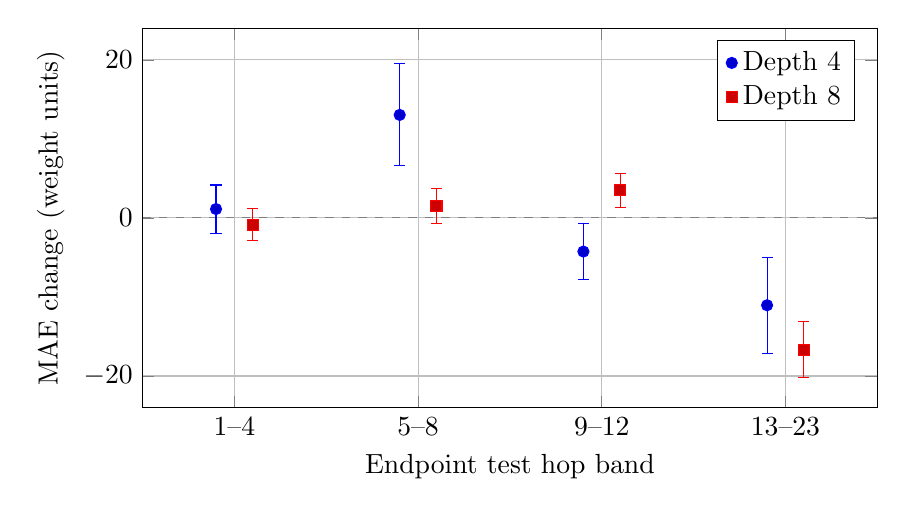
\begin{tikzpicture}
\begin{axis}[width=.9\linewidth,height=6.4cm,xmin=.5,xmax=4.5,ymin=-24,ymax=24,
xtick={1,2,3,4},xticklabels={1--4,5--8,9--12,13--23},
xlabel={Endpoint test hop band},ylabel={MAE change (weight units)},
grid=major,legend pos=north east]
\addplot[gray,dashed,forget plot] coordinates {(.5,0) (4.5,0)};
\addplot+[only marks,mark=*,error bars/.cd,y dir=both,y explicit] coordinates {(0.9,1.124732) +- (0,3.045306) (1.9,13.032529) +- (0,6.452472) (2.9,-4.254731) +- (0,3.559219) (3.9,-11.048670) +- (0,6.051539)};
\addlegendentry{Depth 4}
\addplot+[only marks,mark=square*,error bars/.cd,y dir=both,y explicit] coordinates {(1.1,-0.854376) +- (0,2.042126) (2.1,1.541189) +- (0,2.212262) (3.1,3.485897) +- (0,2.141352) (4.1,-16.659577) +- (0,3.521214)};
\addlegendentry{Depth 8}

\end{axis}
\end{tikzpicture}
\caption{Endpoint minus center training MAE on endpoint queries. Whiskers show one sample SD of paired differences across five replicates. Each replicate contributes 64, 64, 64 and 176 nodes to the respective bands.}
\label{fig:path}
\end{figure}

Endpoint training reduced endpoint test error at hops 13--23 by \(11.05\pm6.05\) at depth four and \(16.66\pm3.52\) at depth eight (Figure~\ref{fig:path}). At both depths those nodes are outside source reach. Endpoint training increased overall center-probe MAE by \(5.96\pm2.24\) and \(3.81\pm0.55\), respectively. With endpoint training fixed, depth eight helped most in the newly reachable 5--8 band, helped at 13--23, and worsened mean error at 9--12. Paired differences are computed before rounding.

\section{Discussion}
The source-swap bound applies to indistinguishable queries on a fixed graph. Empirical MAE also includes distinguishable queries. Beyond source reach, different fitted parameters and additional structural context can still change predictions. Endpoint training jointly shifts the hop and label distributions and the prior over source positions. These shifts could change typical predictions conditional on local structure.

Both raw and normalized MAE support the size hypothesis at the largest size. The family comparison leaves the causes of transfer differences unresolved. Hop-band results give mixed support for a gain specific to newly reachable nodes. The small depth-eight validation contrast fails to predict the direction of the mean large-graph contrast. The tested additive skip shows no consistent benefit across the architectures and optimizer budgets studied.

\section{Limitations and future work}
Five paired replicates support descriptive summaries. The joint data and training seeds do not partition uncertainty, and node observations within a graph are dependent. Structured probes repeat shapes, the controlled path study uses one topology, and random draws are conditioned on connectivity. Width, runtime and convergence remain unresolved in the depth comparison. Larger targets and shifted source distributions can interact with extrapolation. Future controlled studies could independently vary data and training seeds, match hop and weighted-distance support across families, and compare training budgets at equal wall time. Trace supervision and shared recurrent rounds would support a separate investigation of algorithm execution. Representation and sensitivity diagnostics would be required to test oversmoothing or oversquashing.

\section{Conclusion}
Fixed-depth local message passing cannot recover arbitrary weighted distances from a source flag alone. Held-out accuracy can still vary with depth and training-source placement beyond the model's source reach.

\begin{thebibliography}{9}
\setlength{\itemsep}{2pt}
\setlength{\parsep}{0pt}
\bibitem{dijkstra} E. W. Dijkstra. A note on two problems in connexion with graphs. \emph{Numerische Mathematik}, 1:269--271, 1959. \url{https://doi.org/10.1007/BF01386390}
\bibitem{gilmer} J. Gilmer, S. S. Schoenholz, P. F. Riley, O. Vinyals, and G. E. Dahl. Neural message passing for quantum chemistry. \emph{ICML}, PMLR 70:1263--1272, 2017. \url{https://proceedings.mlr.press/v70/gilmer17a.html}
\bibitem{xu} K. Xu, W. Hu, J. Leskovec, and S. Jegelka. How powerful are graph neural networks? \emph{ICLR}, 2019. \url{https://arxiv.org/abs/1810.00826}
\bibitem{yehudai} G. Yehudai, E. Fetaya, E. Meirom, G. Chechik, and H. Maron. From local structures to size generalization in graph neural networks. \emph{ICML}, PMLR 139:11975--11986, 2021. \url{https://proceedings.mlr.press/v139/yehudai21a.html}
\bibitem{execution} P. Veli\v{c}kovi\'c, R. Ying, M. Padovano, R. Hadsell, and C. Blundell. Neural execution of graph algorithms. \emph{ICLR}, 2020. \url{https://arxiv.org/abs/1910.10593}
\bibitem{clrs} P. Veli\v{c}kovi\'c, A. Puigdom\`enech Badia, D. Budden, R. Pascanu, A. Banino, M. Dashevskiy, R. Hadsell, and C. Blundell. The CLRS algorithmic reasoning benchmark. \emph{ICML}, PMLR 162:22084--22102, 2022. \url{https://proceedings.mlr.press/v162/velickovic22a.html}
\bibitem{oono} K. Oono and T. Suzuki. Graph neural networks exponentially lose expressive power for node classification. \emph{ICLR}, 2020. \url{https://arxiv.org/abs/1905.10947}
\bibitem{alon} U. Alon and E. Yahav. On the bottleneck of graph neural networks and its practical implications. \emph{ICLR}, 2021. \url{https://arxiv.org/abs/2006.05205}
\end{thebibliography}

\appendix
\section{Budget and reproducibility details}
For width \(h\) and depth \(k\), the parameter count is \(3h+1+k(5h^2+5h)\), including biases. With \(n\) vertices and \(m\) undirected edges, the dense forward multiply-accumulate proxy is
\[
2nh+k[2m(2h^2+h)+3nh^2].
\]
The terms account for encoder and readout, both message maps per directed edge, and both update maps per vertex. The proxy omits bias, nonlinearities, aggregation, backward computation and optimizer overhead.

The archive records Python 3.12.14, PyTorch 2.15.0+cpu and NetworkX 3.4.2. The main studies used one CPU thread. Archive JSONL records store manifests, epoch curves, predictions and intervention results. The repository reproduction commands use fresh filenames. The paper data script independently checks graph and macro metrics against saved node predictions and emits the table rows and figure coordinates. A SHA-256 manifest records the local archive used for the paper.
\end{document}
